The \gls{EPICS} and related toolkits can be used to control large experiments or even beam lines, but also smaller experimental setups, in which only limited functionalities are needed (e.g., data visualization, archiver, and database). In order to evaluate the hardware that should be used for the final experiment, many relatively (few hundreds of \glspl{PV}) small R\&D setups were built and operated. %Furthermore, harsh ambient conditions inside the STS impose even more rigorous limits. To address the needs of this dynamic environment, a container-based control framework was implemented. 
The two following sections introduce the applications of the developed software package for effective control and data acquisition in two chosen setups. The first section focuses on the powering units irradiation studies and implications for the \gls{STS}. Subsequently, the results from the thermal cycling measurements for the \gls{STS} electronics will be presented and discussed. The thermal cycling studies aimed to discover operational limitations of the \gls{FEE}. 


\section{Irradiation studies of the powering units}

Radiation-induced effects in electronics play an important role in accelerator facilities. Depending on many factors, i.a. location of the setup, intensity, or energy of the incident particles, damage caused to a semiconductor device may vary greatly. A particle could cause no observable effect, transient disruption of circuit operation, a change of logic state, or even permanent damage to the device or integrated circuit (IC)~\cite{dodd}. Hence, studies on the radiation hardness of the devices used for the \gls{CBM} experiment are crucial before choosing the final hardware and its exact position.

One of the detector services that is going to be exposed to the elevated level of radiation is the low voltage powering of electronics. The \gls{STS} will be powered by about 140 low voltage modules, 16 
channels each providing 2100 power channels. In order to estimate the Single Event Effects (\gls{SEE}) in the powering electronics in the envisaged radiation environment, two irradiation campaigns took place in \gls{GSI}, Darmstadt.  The first one was conducted at the mini-CBM experiment and the second was realized next to the electrostatic septum of the SIS18 synchrotron. These irradiation campaigns aimed at detecting radiation-induced soft errors. Soft errors are transient faults in semiconductor devices caused by external radiation, such as energetic particles and cosmic rays~\cite{6338321} in the power units electronics and estimating its rate.

A radiation-induced failure in the low voltage powering of the FEE may lead to a rapid decrease of temperature, as the primary coolant temperature may reach down to \SI{-40}{\celsius}, consequently making the FEE susceptible to thermal stress. The effects of radiation must be therefore studied to ensure the safe operation of the \gls{STS}. Estimation of the soft error rate (\gls{SER}) is critical for the smooth operation of the experiment.

\subsection{FLUKA results as the motivation for the irradiation}

All low-voltage power supplies will be placed in a shielded area within the experimental cave. The estimated dose values were calculated using FLUKA code\footnote{FLUKA is a fully integrated particle physics Monte Carlo simulation package.} and are summarized in Figure~\ref{fig:mCBM})~\cite{FLUKA}. 

\begin{figure}[!h]
    \centering
   % 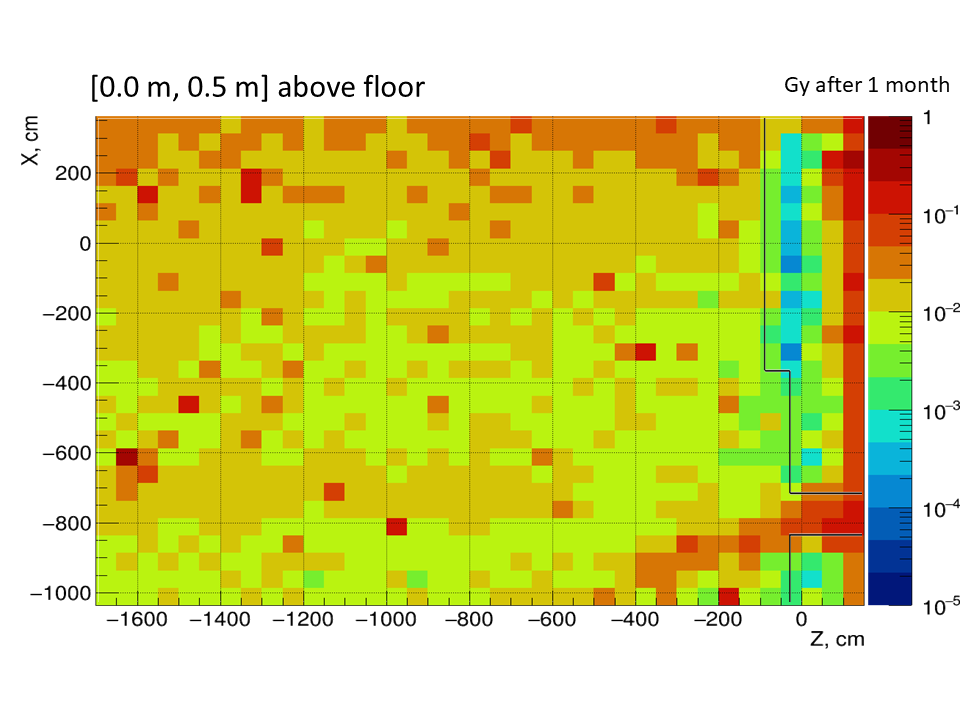
\includegraphics[width=0.95\columnwidth]{images/dose3.png}
    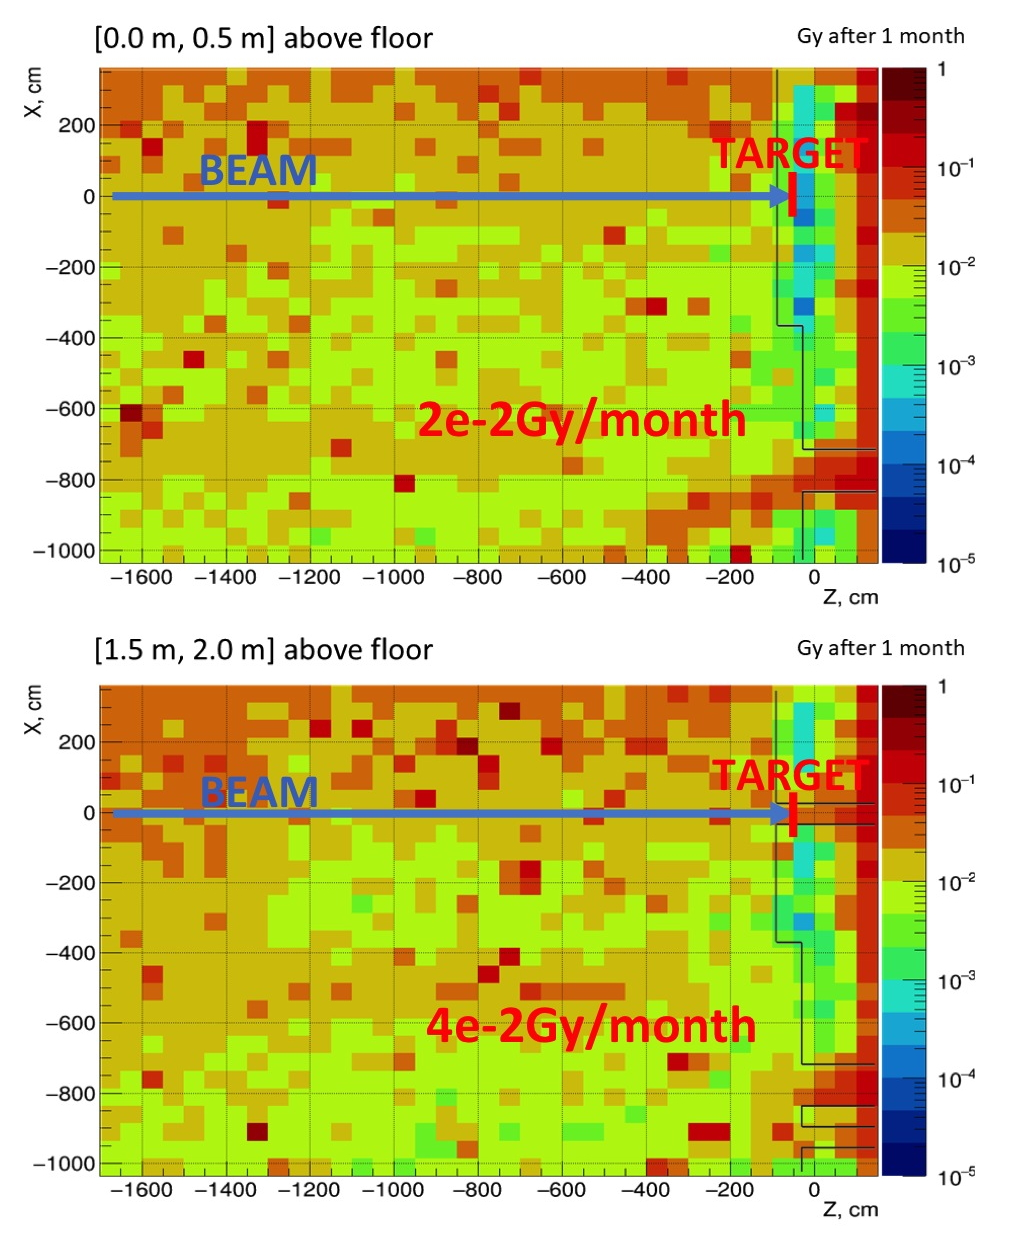
\includegraphics[width=0.7\columnwidth]{Chapter4/images/Dose00.jpg}
    \caption{Expected dose distribution in the air in the \gls{CBM}
cave under the platform (\agev{11} Au $10^{9} \mathrm{\ ions/s}$ on 1\% Au
interaction target). The first simulation depicts the radiation doses at heights between 0 and \SI{0.5}{\metre} and the second one from \SI{1.5}{\metre} to \SI{2}{\metre}~\cite{fluka_senger}.} 
    \label{fig:mCBM}
\end{figure}
%newpage
For Au beams with the highest available intensities 
($10^{9}\,$\ionss) and energies 
(\agev{11}), a total dose\footnote{Gray is a SI unit of ionizing radiation dose, defined as the absorption of one joule of radiation energy per kilogram of matter \cite{gray}.} of \mgy{20} is expected after 1 month of operation in the area between 0 and \SI{0.5}{\metre} above the ground (at the planned location of the power crates x = \SI{-600}{\centi\metre}, z = \SI{-600}{\centi\metre}) and \mgy{40} between \SI{1.5}{\metre} and \SI{2}{\metre} above the ground (x = \SI{-600}{\centi\metre}, z = \SI{-600}{\centi\metre}).
 


\subsection{Single Event Effects in electronics}

A variety of different elements and chemical compounds can be used in electronics, including silicon, silicon dioxide ($\mathrm{SiO}_{2}$), or boron. The high ambient flux of particles in a particle accelerator environment usually consists of charged particles (mostly protons, and electrons), high-energy photons (gamma and X-rays), and a broad spectrum of neutrons.

 Radiation-induced soft errors have become a huge concern in advanced computer chips because uncorrected, they produce a failure rate that is higher than all the other mechanisms compromising reliability combined~\cite{1545891}. These kinds of errors are especially important for high energy physics and aerospace applications, as it may severely affect the reliability of electronics components. Moreover, cumulative radiation effects occur during the complete lifetime of a transistor as long as it is exposed to radiation~\cite{RodriguezRodriguez2020}.

Different interaction mechanisms may cause both stochastic and deterministic effects in electronics. These effects are directly related to the integrated dose and linear energy transfer (\gls{LET}) of the incident particles~\cite{electronic_system_on_module}.  LET is defined as the energy absorbed in matter per unit path length travelled by a charged particle
\begin{equation}
    L = \frac{dE_{abs}}{dx}.
\end{equation}
The charged particles generate electron-hole pairs on the particle track and deposits charge. The generated charge is collected to the drain by drift and diffusion, and causes soft error. These effects are usually local, but they may propagate through the whole system. The most common mechanisms responsible for the soft errors are transient effects and static effects (related to content change in a memory cell). 

On the other hand, neutrons do not cause direct ionization in silicon or oxygen. These neutral particles interact elastically as well as inelastically, resulting either in the creation of other nuclei and emission of a light particle or in changes in the kinetic energies of the participants. A few neutron threshold energies for reactions with oxygen and silicon are summarized in Table~\ref{cross-seciton}. The cross-section for neutron reactions generally decreases with the energy. Moreover, neutrons can indirectly cause \gls{SEE} by secondary radiation, for example, a reaction with boron which results in the emission of an $\alpha$ particle $\mathrm{^{10}B(n,\alpha)^{7}Li}$~\cite{1545891,neutrons_energy,neutrons_energy_2}. 

\begin{table}[!h]
\centering
\caption{Threshold energies of neutron reactions with silicon and oxygen nuclei~\cite{ENDF}.}
\begin{tabular}{lc}
\hline
Reaction         & Neutron Threshold Energy (MeV) \\ \hline
Si elastic       & 0                              \\
Si(n,$\alpha$)   & 2.75                           \\
Si(n,p)          & 4                              \\
Si(n,d)          & 10.5                           \\
Si(n,$n-\alpha$) & 10.35                          \\ \hline
O elastic        & 0                              \\
O(n,$\alpha$)    & 2.35                           \\
O(n,$n-\alpha$)  & 7.61                           \\
O(n,p)           & 10.24                          \\
O(n,d)           & 10.53                         
\end{tabular}

\label{cross-seciton}
\end{table}

% Write a summary about the cross section etc that in case of CBM and this chapter we want to use realistic conditions to check behavior of the 

%\newpage
\subsection{Methodology}

The subject of the irradiation campaigns was a MPOD mini crate with one low voltage (WIENER~\cite{wiener}) and one high voltage (ISEG~\cite{iseg}) module. The crate CC24 controller (ISEG) offers an embedded \gls{EPICS} Input Output controller, which was used to detect radiation-induced channel or module failures. All registered  failure events were stored in a dedicated database.  

In order to correlate the soft failure rate with the absorbed dose, two types of thermoluminescent dosimeters were used. A larger polyethylene sphere (d = 30\,cm) allowed measuring the neutron ambient dose, whilst the cylinder (d = 5\,cm, h = 6\,cm) measured other particles~\cite{bonner}. We assume that the conditions (e.g., neutron spectra) at the \gls{CBM} experiment will be similar to conditions at SIS18, and at the \gls{mCBM} experiment. The quality factor sets the relation between \gls{LET} and relative biological effectiveness (\gls{RBE}). It converts the measured dose given in sievert to absorbed energy in gray. It is assumed that the factor equals 5 for sphere in both irradiation campaigns. The dose measured with the cylinder is assumed to have a quality factor of 1.

\subsection{Low statistics data analysis}

We assume that failure events (radiation-induced soft errors) are statistically independent and are driven by purely stochastic factors. In addition, we take into account only the total dose measured by the dosimeters, thus rapid dose changes and their effect are not investigated in this contribution. In such a case, the probability of observing $n_{m}$ events with the mean value $\mu$ is described by the Poisson distribution\newline
\begin{equation}
    p(n|\mu) = \frac{\mu^{n}}{n!}e^{-\mu}.
\end{equation}
The total number of events is considered to be the average $\mu$. Considering 68\% confidence levels for values $n_{m} > 2$ we can apply the following equations to estimate the distribution bands (see Figure~\ref{fig:poisson})~\cite{schmidt}.

If in an experiment $\mu$ events are measured, we conclude that the standard deviation is described by $\mu - \sqrt{\mu}$ and $\mu + 1 + \sqrt{\mu}$ around the average value $\mu$.

\begin{figure}[!h]
    \centering
    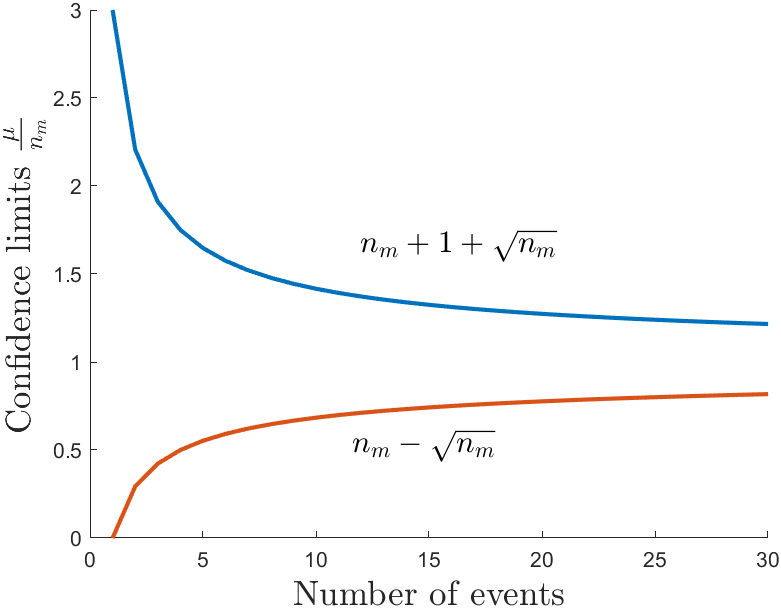
\includegraphics[width=0.55\columnwidth]{Chapter4/images/poisson.png}
    \caption{Estimated bands of the Poisson distribution~\cite{schmidt}.}
    \label{fig:poisson}
\end{figure}
%\newpage

For $n_{m} \leq 2$ previously mentioned, estimations do not provide accurate results, therefore upper and lower bands need to be calculated explicitly. According to~\cite{schmidt}:



\begin{table}[!h]
\centering
\caption{Estimated bands of the Poisson distribution for low number of events $n_{m}  \leq 2$.}
\begin{tabular}{ccc}
\hline
Number of counts & \multicolumn{2}{c}{Poisonn distribution} \\ \cline{2-3} 
$n_{m}$          & $\mu_{l}$            & $\mu_{u}$           \\ \hline
0                & 0                    & 1.84                \\
1                & 0.17                & 3.30                \\
2                & 0.71                & 4.64                \\ \hline
\end{tabular}
\end{table}
%\newpage
\subsection{Irradiation at the mCBM experiment}
In order to investigate electronics operation under the realistic conditions, that low voltage modules will face during the CBM experiment, an irradiation campaign took place at the \gls{mCBM} experiment (see figure~\ref{fig:CBM1}). Different intensities and reaction systems (Au+Au, Au+Ni, etc.) were exercised during the experiment.
\begin{figure}[!h]
    \centering
    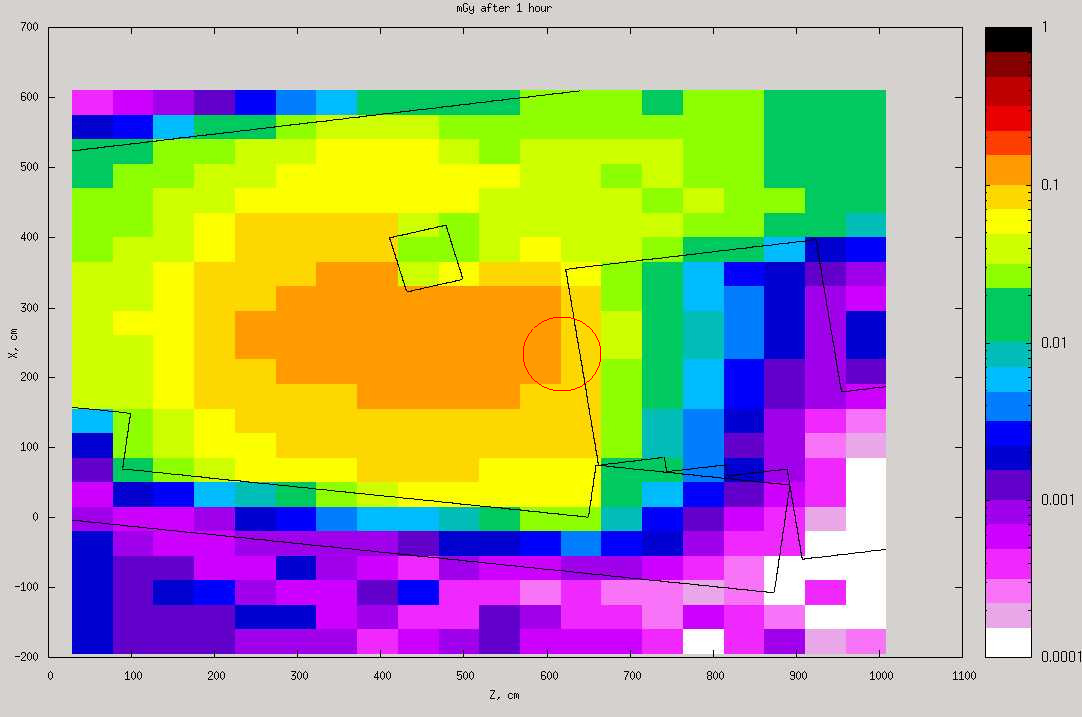
\includegraphics[width=0.65\columnwidth]{Chapter4/images/dose1.jpg}
    \caption{Expected dose rate distribution (mGy/hour) in the \gls{mCBM} cave with 2 AGeV O ions beam of $10^{7}\mathrm{\ ions/s}$ on 4 mm Ni target. In the encircled area the dose reached about 0.1\,mGy/hour~\cite{fluka_senger}.}
     \label{fig:CBM1}
\end{figure}


To measure the dose that the crate was exposed to, four thermoluminescent dosimeters (\gls{TLD}) with moderators were used (Figure~\ref{fig:crate}). Two of these TLDs were as positioned in the background as can be seen in Figure~\ref{fig:crate}, and they served as a reference. Two remaining dosimeters were located next to the irradiated crate. During the irradiation at the \gls{mCBM} experiment, the dosimeters were read out twice, in order to evaluate the total dose received by the crate. The first value was $19.72\mathrm{\ mGy}$ and  the second one was $72.31\mathrm{\ mGy}$. 


\newpage
\begin{figure}[!h]
    \centering
    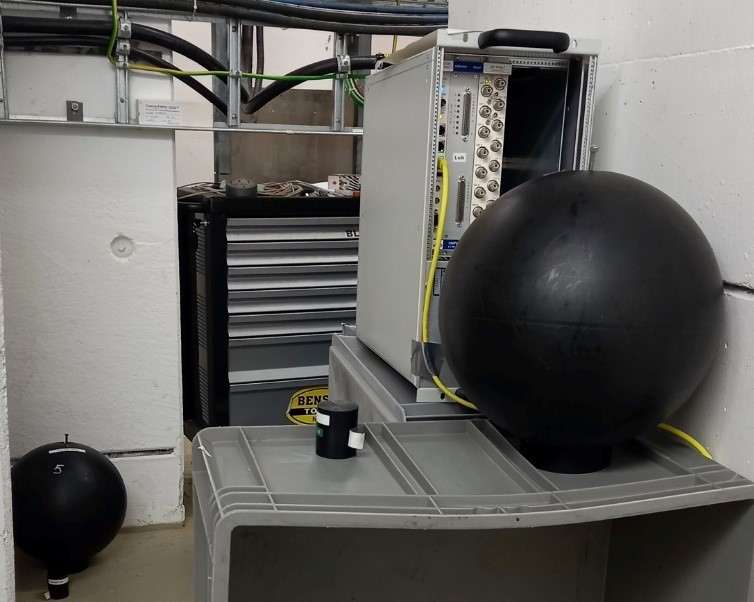
\includegraphics[width=0.5\columnwidth]{Chapter4/images/crate.jpg}
    \caption{Crate irradiation setup at the \gls{mCBM} experiment. The photo depicts two TLD dosimeters in the background, and two TLD dosimeters and the crate in the foreground.}
    \label{fig:crate}
\end{figure}

A \gls{SEE} in the low voltage module occurred in each part of the irradiation. In both cases, it was possible to recover the functionalities by enabling the channels again. After applying lower and upper limits according to the Poisonn distribution
%\newpage

\begin{equation}
    D_{lower}=\frac{92}{0.708} = 129.9\mathrm{\ mGy}
\end{equation}
\begin{equation}
    D_{upper}=\frac{92}{4.64} = 19.8\mathrm{\ mGy}.
\end{equation}

The uncertainty for $n_{m}=2$ is extremely high and equals to $\mathrm{46}_{-26}^{+84}$\,mGy, therefore no clear conclusion on the behavior of the crate could be made. To further increase the statistics, a second irradiation campaign took place at the electrostatic septum of the SIS18 synchrotron. 

%\vspace{10cm}
\subsection{Irradiation at the SIS18 septum}
\subsubsection{Setup description}
The setup at the SIS18 septum consisted of two \gls{TLD} dosimeters (for neutrons and other particles separately). Furthermore, the total doses from TLDs were supplemented with readouts from two active dosimeters placed behind the wall (see Figure~\ref{fig:spec_des}). These dosimeters were used to assess the influence of the dose rate on the \gls{SEE}.
\begin{figure}[!ht]
    \centering
    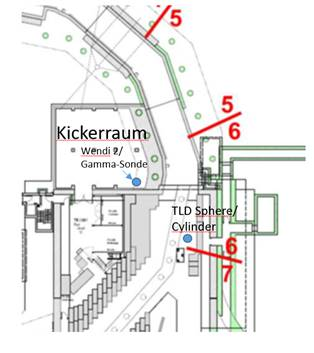
\includegraphics[width=0.45\columnwidth]{Chapter4/images/septum.jpg}
    \caption{Location of the dosimeters and crate at the SIS18. The so-called Kickerraum contained WENDI-2 and Gamma probe, whereas two TLD dosimeters were placed next to the power crate - depicted with a blue dot between segments 6 and 7.}
    \label{fig:spec_des}
\end{figure}

Wendi-2 is a precise wide-energy neutron dosimeter~\cite{wendi} that was used to determine the neutron dose rate in the so-called Kickerraum (Figure~\ref{fig:spec_des}). Due to the shielding of the wall, the gamma probe measured mostly background radiation. The MPOD mini crate was placed next to the TLD dosimeters. In order to calculate the momentary neutron dose next to the crate, a ratio of total doses from both measurement places was used. 
\newpage
\subsubsection{Results}
During the irradiation period, readings from the dosimeters reached $106.1\mathrm{\ mSv}$ and $27.7\mathrm{\ mSv}$ for neutrons and other particles respectively.
%(Figure~\ref{fig:spectrum} depicts neutrons spectrum at the irradiation place).
%\begin{figure}[!ht]
%    \centering
%    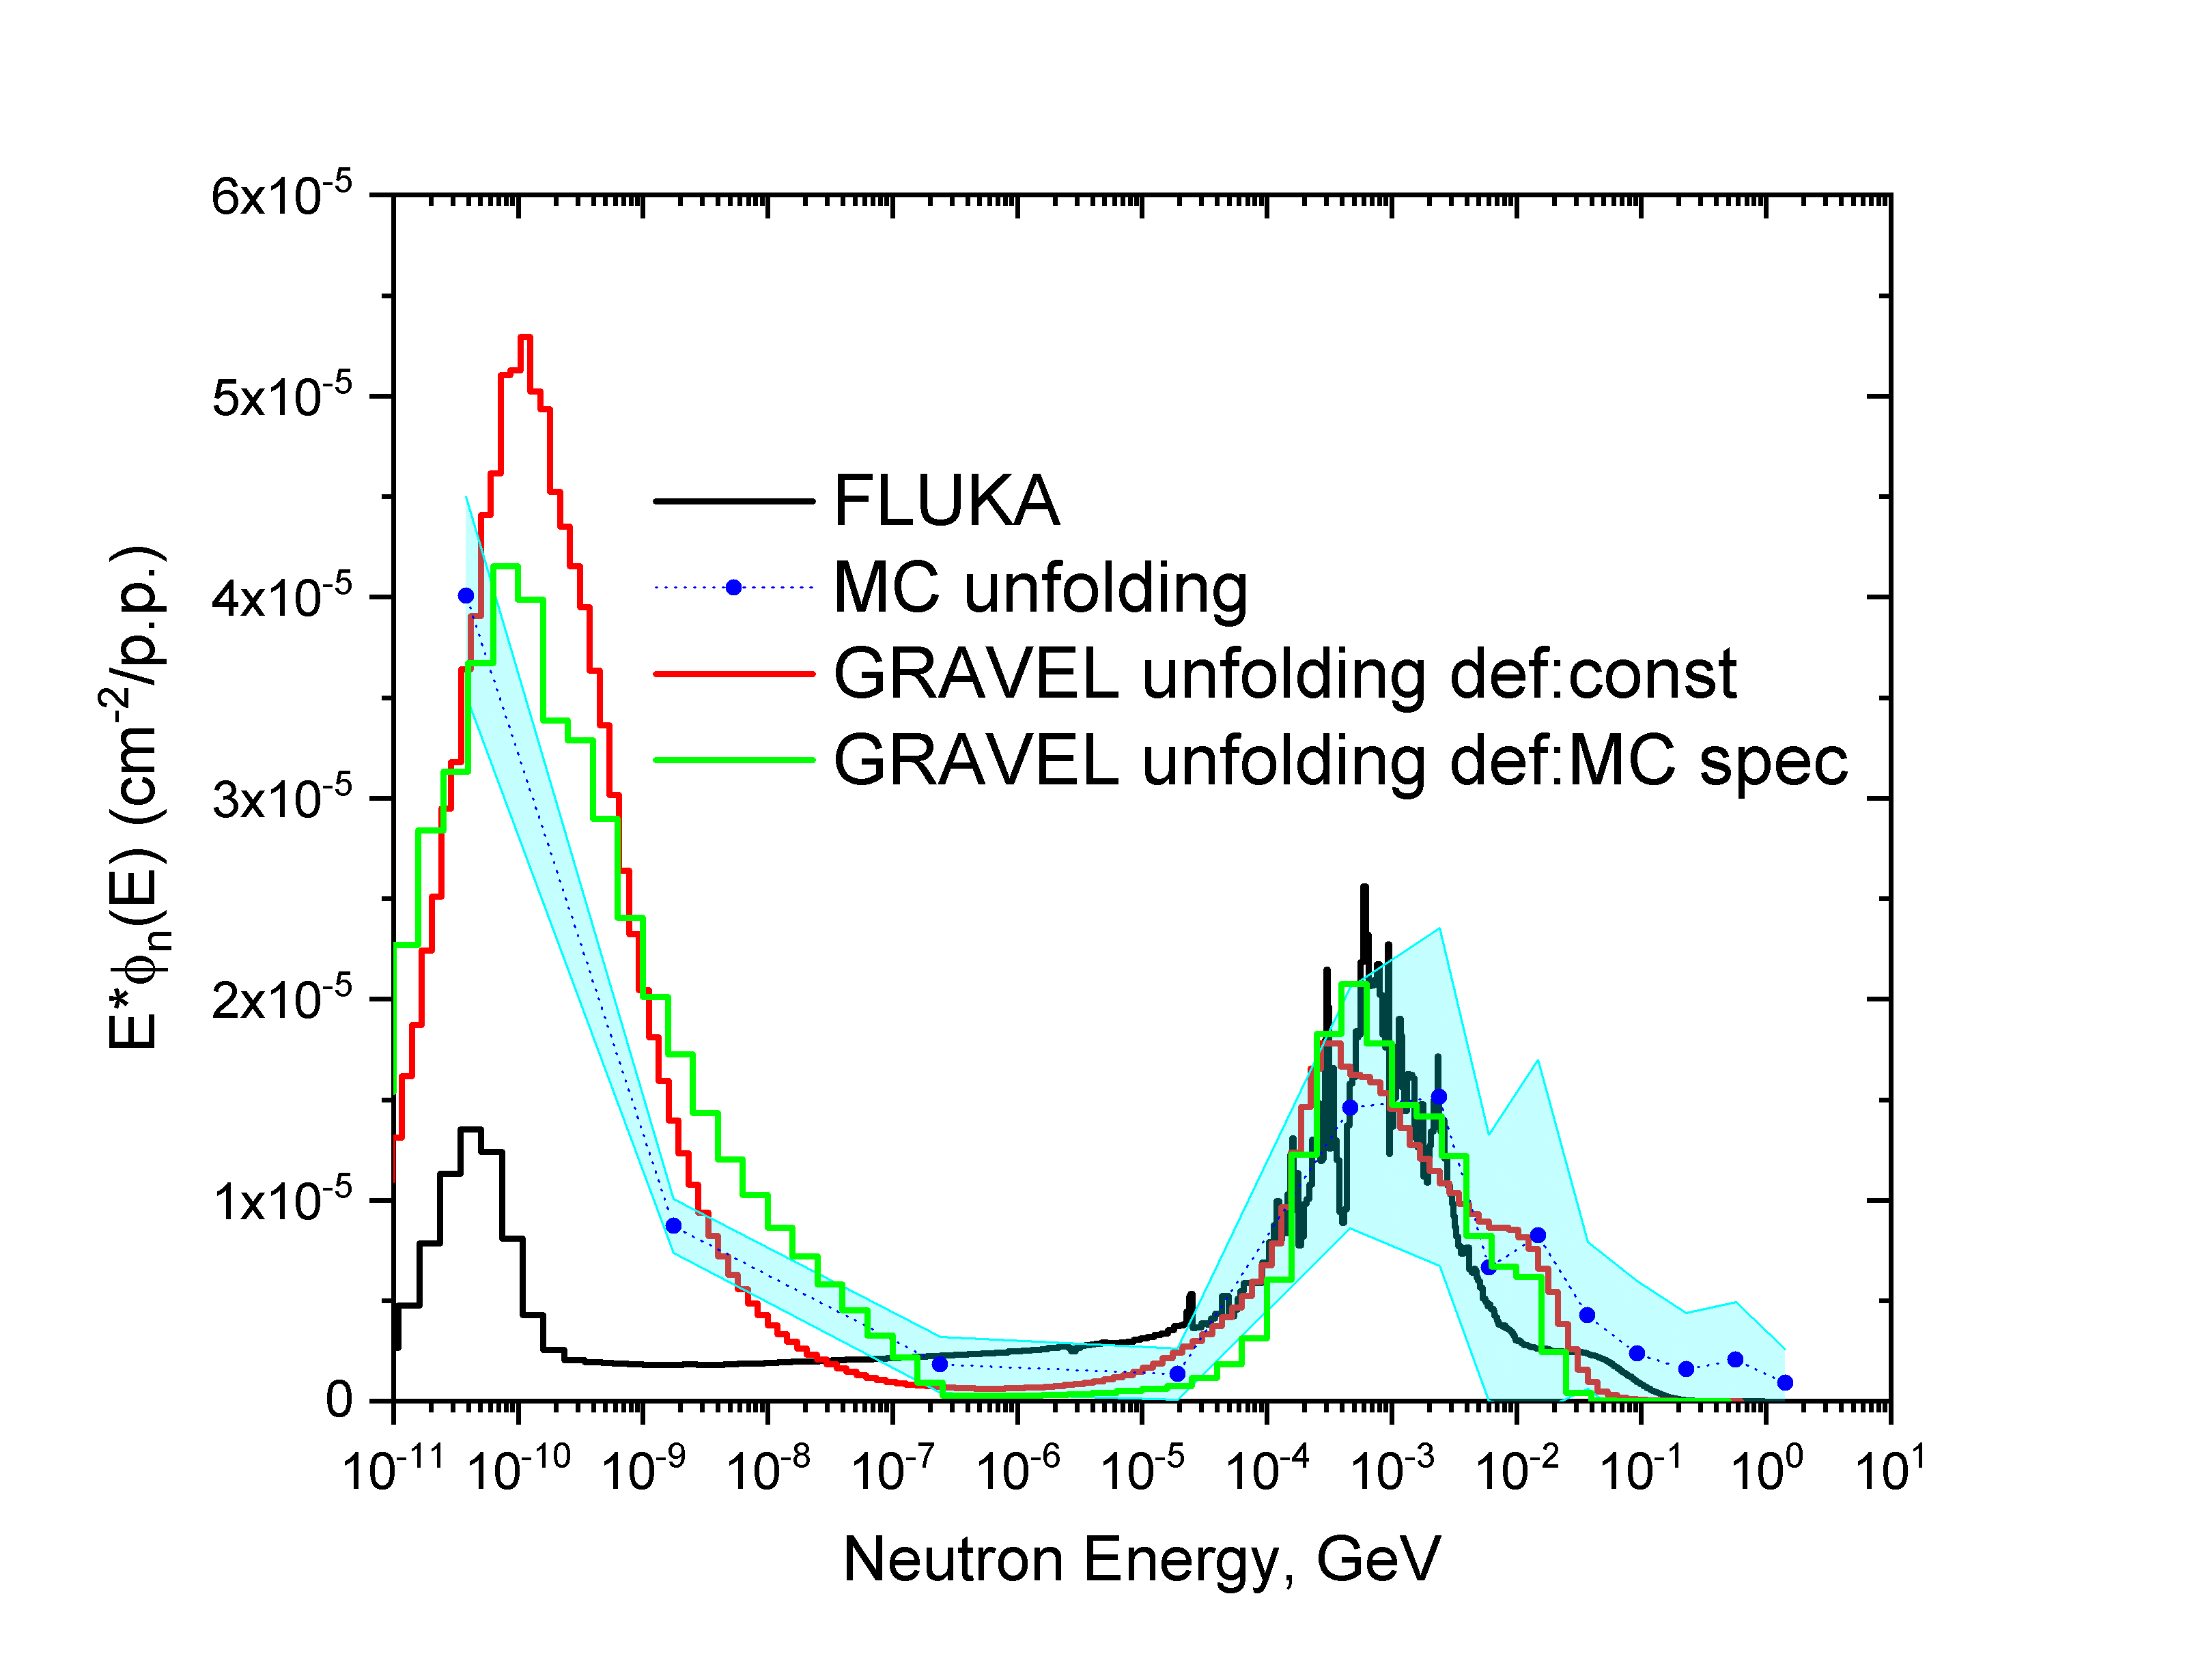
\includegraphics[width=0.9\columnwidth]{Chapter4/images/fig5.png}
%    \caption{Neutron spectrum at the measurement location (SIS18 septum). It is based on the measurement of argon ions at 550 MeV/u. The first peak is related to the thermal neutrons and %the second one to the fast neutrons}
%    \label{fig:spectrum}
%\end{figure}
Using assumed quality factors, the ambient dose was converted to the absorbed dose values. Hence, we get in total $49\pm{2}\mathrm{\ mGy}$, taking into account 5\% standard uncertainty of the TLD dosimeters. During the test, 11 radiation-induced soft failures were identified in the low voltage module. Therefore, it is possible to estimate an average dose after which a low voltage failure might take place.
\begin{figure}[!h]
    \centering
    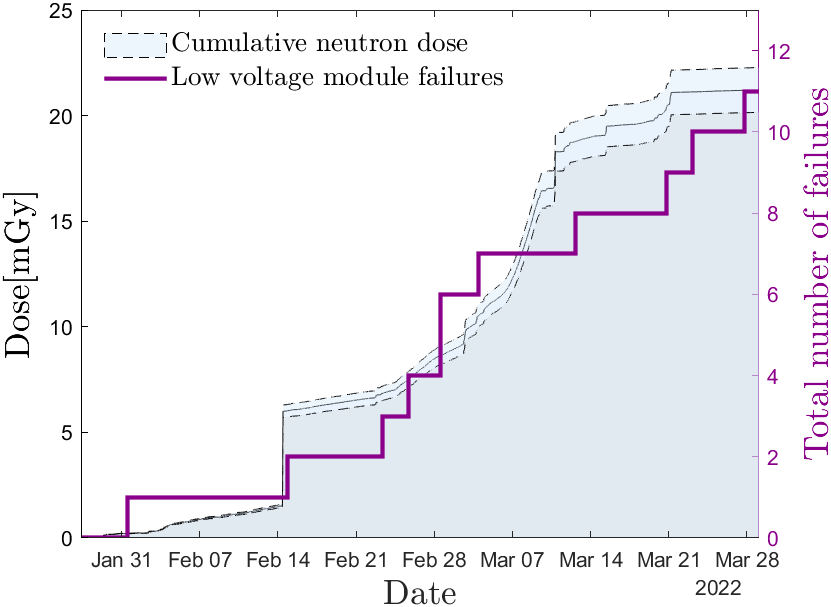
\includegraphics[width=0.6\columnwidth]{Chapter4/images/LV_failure_and_neutronsrate.png}
    \caption{Cumulative neutron dose and \gls{SEE} in the low voltage module.}
    \label{fig:lv_neutrons}
\end{figure}
\begin{figure}[!h]
    \centering
    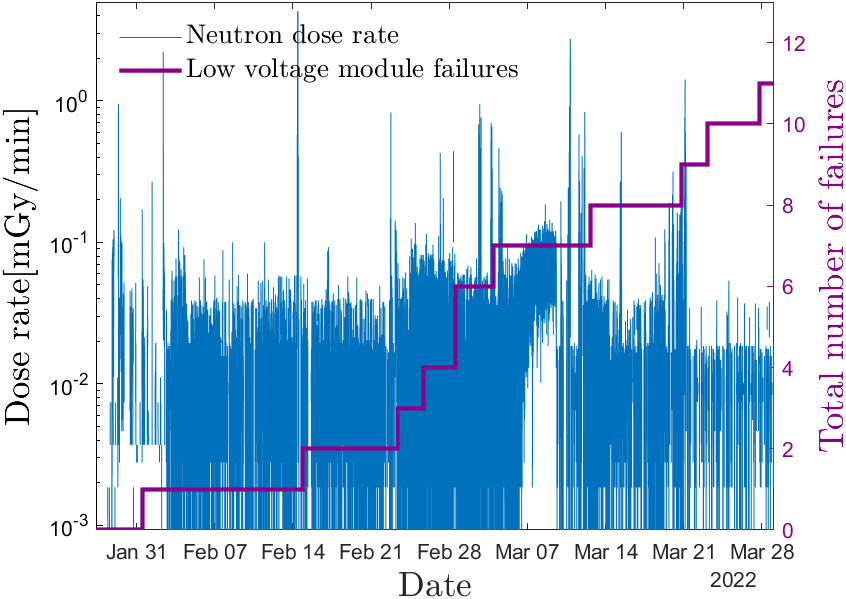
\includegraphics[width=0.6\columnwidth]{Chapter4/images/neutrons_dose_rate.png}
    \caption{Neutron dose rate and failures of the low voltage module.}
    \label{fig:lv_neutrons_rate}
\end{figure}
Figure~\ref{fig:lv_neutrons} shows how the number of failures cumulate with the total neutron dose, where the longer periods without failure indicate a break in SIS18 operation. Similarly, Figure~\ref{fig:lv_neutrons_rate} depicts the dose rate and related \gls{SEE}.
For the 11 low voltage module failures, the confidence bands from the Poisson distribution are as follows
   \begin{equation}
  \mathrm{\mu}_{\mathrm{LV}}^{\mathrm{SEE}}=\mathrm{11}_{-3}^{+4}.
\end{equation}
Considering the sum of two doses $49\pm{2}\mathrm{\ mGy}$, a soft error occurs after
\begin{equation}
    \mathrm{D}_{\mathrm{LV}}^{\mathrm{SEE}}=\mathrm{4.45}_{-1.25}^{+1.93}\mathrm{\,mGy}.
\end{equation}
After the occurrence of a soft error in the low voltage module, it was always possible to turn the channels on again.

The high voltage modules will be placed outside the cave in an area with lower radiation levels, thus their error sensitivity does not pose a risk to detector operation. In the case of the high voltage module, the \gls{SEE} do not result in a module switch off, but in disabling channels. In two cases, all channels were switched off, which is counted as if 16 channels were turned off at the same time. Figure \ref{fig:hv_neutrons} and \ref{fig:hv_neutrons_rate} show the channels failure rate with the increasing cumulative dose. 
\begin{figure}[!h]
    \centering
    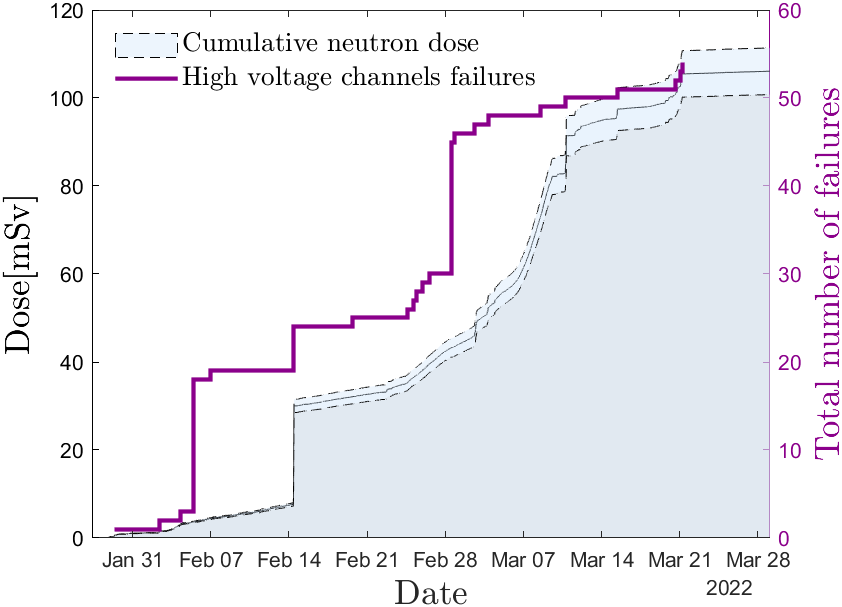
\includegraphics[width=0.6\columnwidth]{Chapter4/images/HV_failure_and_neutronrate.png}
    \caption{Cumulative neutron dose and failures of the high voltage module channels.}
    \label{fig:hv_neutrons}
\end{figure}
\begin{figure}[!h]
    \centering
    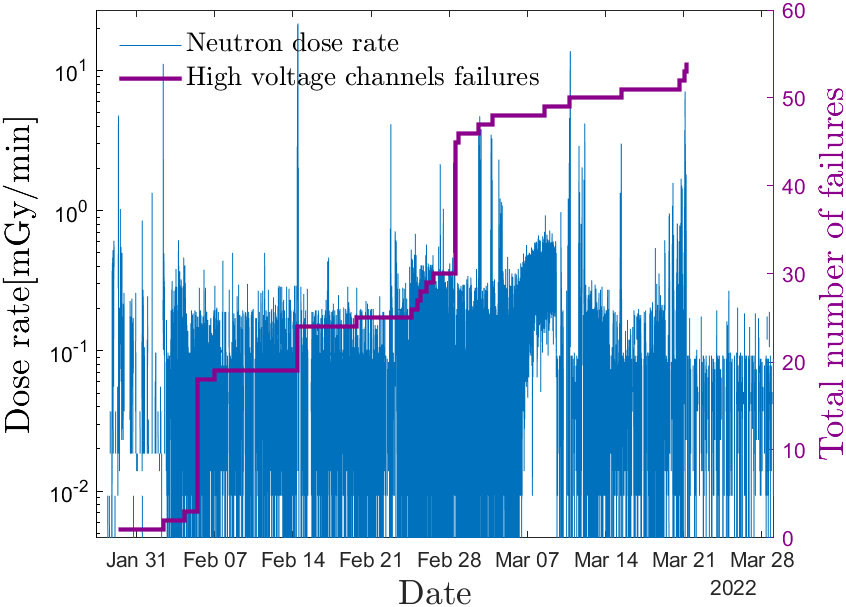
\includegraphics[width=0.6\columnwidth]{Chapter4/images/Hv_neutrons_dose_rate.png}
    \caption{Neutron dose rate and failures of the high voltage module channels.}
    \label{fig:hv_neutrons_rate}
\end{figure}
For the high voltage module, the total number of channels that switched off due to the irradiation is 56. Following a similar procedure as for the previous calculation
  \begin{equation}
 \mathrm{\mu}_{\mathrm{HV}}^{\mathrm{SEE}}=\mathrm{56}_{-7}^{+8}.
\end{equation}
Considering the failure number, it translates to
\begin{equation}
    \mathrm{D}_{\mathrm{HV}}^{\mathrm{SEE}}=\mathrm{0.88}_{-0.12}^{+0.13}\mathrm{\,mGy}.
\end{equation}
If the high voltage module was situated in the same place as the low voltage, a channel switch off could happen after $\mathrm{0.88}_{-0.12}^{+0.13}\mathrm{\,mGy}$.

\subsection{Conclusions}

\label{irradiation_results}
The control framework introduced in the previous chapter served as the data acquisition system for the irradiation of the MPOD crate and two modules. Prepared graphical user interfaces together with archiver, database allowed to track the failure events and compare them later on with the registered dose. Obtained results have a direct influence on the experiment operation.

The \gls{FEE} of the \gls{STS} will be powered by about 140 low voltage modules. Given that in the worst case, some of those modules will be exposed to about 40\,mGy/month, the measurement indicates that about 9 \gls{SEE} per month per module will occur. In practice, it means that every \gls{FEB} will need to withstand 9 power cycles at low temperatures per month. Assuming operation of 2 months per year and a total projected operating time of 10 years, electronics must withstand at least 180 power cycles at low temperatures of about \SI{-20}{\celsius}.
\subsection{Potential risk to STS operation}
If every low voltage module turns off 9 times per month during the operation, the potential consequences need to be carefully assessed. By planning the powering scheme for the \gls{STS}, the system can be prepared for the foreseen power interruptions. In the worst-case scenario, considering 140 low voltage modules,  about 1260 soft errors a month, which corresponds to 1.75 errors per hour.  For the 16 \glspl{ROB} connected to one low voltage module, a temporary shutdown of up to 140 \glspl{FEB} or 70 modules per hour is expected.  The duration of the shutdown is also critical for the operation. A soft error in the low voltage module can most likely be recovered within seconds, preventing extensive thermal stress in the \gls{FEE}. On the other hand, for the testing scenarios, it is necessary to consider that the electronics experience full thermal stress, in case fast power recovery is not possible. Additionally, power cycles of the \gls{FEE} in low temperatures may result in thermally induced mechanical stresses on the components of the Printed Circuit Boards (\glspl{PCB}). Hence, the effects of thermal cycling of the \gls{FEE} should be carefully studied, in order to evaluate the limits in the performance of the electronics  (see section~\ref{thermal_cycling}). Nevertheless, there are also a few methods to decrease the potential risk, both from the radiation-induced damage and potential problems due to thermal shock:
\begin{itemize}
    \item additional radiation shielding material around the power supplies,
    \item powering scheme - for example connecting \glspl{ROB} and corresponding \glspl{FEB} to the same low voltage module,
    \item proper software/hardware mechanisms to switch on the channels in a matter of seconds.
\end{itemize}
\newpage
